% 相机模型
\pentry{三维投影\upref{proj3D}, 图片坐标系\upref{imgFrm}}

\begin{figure}[ht]
\centering
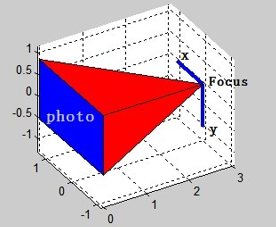
\includegraphics[width=5cm]{./figures/CamMdl_1.png}
\caption{相机坐标系} \label{CamMdl_fig1}
\end{figure}

从焦点出发, 穿过底片并与底片垂直的射线叫做\textbf{光轴}.

以焦点为原点, 光轴方向为 $z$ 轴, 图片的右方为 $x$ 轴, 下方为 $y$ 轴(注意这是常用的右手系\upref{RHRul}).

真实的相机和这里的相机模型存在误差, 通常需要将图片进行纠偏后才能得到符合模型的图像. 以后我们讨论的图像一般指纠偏后的图像.

注意图像的中点不一定是光轴和底片的交点.

相机参数: 焦距, 底片宽度, 底片高度, 光轴的图像坐标

相机的位置参数: 焦点的位置, 三个单位矢量在世界坐标系中的坐标(即旋转矩阵, 也可以使用四元数表示)

反过来, 若已知图片和相机位置和参数, 我们可以将图片上的每一点对应到以相机为起点的一条射线. 而至于这点具体在射线上的什么位置无从得知. 但如果我们从两个不同的位置拍摄同一点, 就可以通过两条射线的交点确定该点位置.

若已知相机参数, 我们可以通过图片中的任意两点确定它们关于相机的夹角(即两条射线的夹角).
